%%==================================================
%% chapter04.tex for SJTU Master Thesis
%% based on CASthesis
%% modified by wei.jianwen@gmail.com
%% version: 0.3a
%% Encoding: UTF-8
%% last update: Dec 5th, 2010
%%==================================================

% \bibliographystyle{sjtu2} %[此处用于每章都生产参考文献]
\raggedbottom
\chapter{DiffCon的设计与实现}
\label{chap:designandimpl}

\section{引言}

前文总结了课题相关的基础算法和优化思路之间的联系和启发,探讨了范围查询需求和算法的数据组织形式之间的关联点,本章节以优化频率矩阵加噪模型、提升发布数据可用性为目的,论述解决方案——非交互式差分隐私匿名优化算法DiffCon的设计和实现。

本章结构安排:首先由基础算法DiffGen的相关特性入手,推导DiffGen具有一维直方图特性的理论基础,证明DiffCon优化方案的可行性和正确性;接着介绍具体的设计实现,基于一致性约束从设计新的应答查询模式、重定义全局敏感性以及噪音调整算法这三个方面介绍DiffCon算法细节,并证明最小二乘法目标式的正确性;然后通过类图描述具体的算法实现;最后进行性能的理论分析与总结。

\section{理论基础及证明}

基于前文对DiffGen算法的论述,本小节先总结了其数据发布模型所具有的相关性质,然后推出DiffGen模型具有一维直方图特性的结论,并给出严谨的证明,为课题所设计的解决方案的可行性和正确性做好铺垫。

\subsection{DiffGen算法的相关特性}

\subsubsection{唯一性}

每个叶节点上的数据项在DiffGen分类树上是唯一出现的,可通过简单的反证法证明。
\begin{prop}
	\label{chap4_prop1}
	(DiffGen算法的唯一性)DiffGen分类树中,叶节点的属性值分布具有唯一性,即在所有叶节点上,不存在相同的两个数据项。
\end{prop}
\begin{proof}
	见附录\ref{proof}。
\end{proof}
此特性决定了针对某一属性范围的节点组合是非冗余的,保证了组合结果的唯一合法性。否则,查询结果会存在二义性问题,使得查询请求返回失败。

\subsubsection{完整性}

\begin{prop}
	\label{chap4_prop2}
	(DiffGen算法的完整性)DiffGen分类树的构建过程中,每次属性的划分具有完整性,即对于某次分裂$v$$\rightarrow$$child(v)$,$child(v)$中的每个属性值在$Cut_{i}$中能够完整更新。
\end{prop}
\begin{proof}
	见附录\ref{proof}。
\end{proof}
属性值分裂的完整性确保了对于合法正常的查询请求,均能在DiffGen分类树中找到相匹配的节点,都能返回应答结果。

\subsubsection{健壮性}

属性划分的完整性确保了在各种合法查询请求中,DiffGen框架的绝对健壮性,首先定义合法查询如下。

\begin{defn}
	(合法查询)有d个属性的数据集,属性$A_{i}$的匿名树上的所有属性值集合为$T_{i}$,$i$ $\in$ [1,d],则所有匿名树的属性值集合$T_{total}$ = $\sum\limits_i^d \cup T_{i}$。
	基于属性值区间的查询能够拆分成若干个属性值的组合,因此某查询请求$Q$可表示成涉及$k$个不同的属性值查询,$Q$=$\{a_{1},a_{2},...,a_{k}\}$,其中k $\leqslant$ |$T_{total}$|,$a_{k}$为属性值。若查询$Q$满足以下条件,则$Q$为合法查询:
	\begin{equation}
	\text{对于}\forall a_{i} \in Q, i \in [1,k], \text{总有}a_{i} \in T_{total}
	\end{equation}
\end{defn}

\begin{prop}
	\label{chap4_prop3}
	(DiffGen算法的健壮性)对于任意的合法查询,DiffGen返回的应答结果具有绝对健壮性,即对于查询序列中的任一属性值查询,均能在DiffGen分类树上找到应答节点。
\end{prop}
\begin{proof}
	见附录\ref{proof}。
\end{proof}

DiffGen框架的健壮性,保障了对于任意的待查询项,在DiffGen分类树中总能找到完整覆盖其属性值的应答节点,达到对于合法查询有求必应的效果,是证明DiffGen框架具有一维直方图特性的关键性质。

\subsubsection{一致性}

\begin{prop}
	\label{chap4_prop4}
	(DiffGen算法的一致性)在DiffGen分类树上,节点上的数据项之间具有一致性特性,可通过节点的组合运算应答合法查询请求。
\end{prop}
\begin{proof}
	见附录\ref{proof}。
\end{proof}

基于分类树结构的健壮性和一致性特性使得对于任一查询项总能找到应答节点或节点集,保证了组合树节点作为应答返回方案的可行性,是替换原有应答模式、设计新查询应答模式的基础

%基于差分隐私的组合性质,在论文\cite{DiffGen}中证明了DiffGen满足$\varepsilon$-差分隐私,并且叶节点数据项之间是相互独立的。

\subsection{一维直方图特性} %正确性讨论,花了这么大力气一堆命题,就是为了说明可利用boost的思路

%最好能搞成命题啊1,范围覆盖,2相互独立(基于差分隐私组合性质)

一维直方图发布模型的特点在于能够响应所有的合法查询请求,对于属性值的范围查询能够通过一系列柱状条的叠加得到,并且单个柱状条计数值的增减改变是不影响其他柱状条的。而在多属性直方图中,随着属性值的增加使得数据集的数据域尺寸变大,柱状条的叠加难以满足所有的合法查询请求,健壮性得不到保障;并且,由于多属性的影响,在属性值的范围查询中每个柱状条之间相互影响,全局敏感性不为1。

\begin{prop}
	\label{chap4_prop5}
	(DiffGen框架的一维直方图特性)DiffGen模型具有一维直方图特性,即在范围查询需求中,DiffGen模型的应答健壮性和发布数据项之间的独立性满足一维直方图特征。
\end{prop}
\begin{proof}
	见附录\ref{proof}。
\end{proof}

本小节对DiffGen算法的唯一性、完整性、健壮性、一致性的性质进行推导,结合差分隐私组合特性最终得出DiffGen算法本质上具有一维直方图特性的结论,说明了采用如$BoostH$的基于一致性约束的优化思路的可行性,进而可设计新的查询应答模式---针对查询范围的搜寻最优节点的覆盖集合。
对于分类应用中的范围计数查询需求,本小节的证明确保了DiffCon优化算法的正确性,一维直方图模型特性和一致性约束是理论基础。


%\section{基于一致性约束的优化算法DiffCon}
\section{优化算法DiffCon的设计与实现}

%从设计新的应答查询模式、重定义全局敏感性以及基于一致性约束的噪音调整算法
针对范围计数查询应用,基于上节的理论证明,本节就一致性约束的优化思路,对非交互式差分隐私优化算法DiffCon的整体设计进行详细阐述。主要分为以下几个部分:
\begin{enumerate}
	\item 立足于DiffGen的分类树结构,构建辅助树结构$DTree$。它是对原数据集进行重匿名、划分,对噪音分布进行优化调整以及定义新的应答查询模式的基础。
	\item 实现基于树结构的最小顶点覆盖集算法TMSC,设计新的应答查询模式,并重定义全局敏感性。TMSC算法是DiffCon应答查询模式的设计和运行基础,是优化原理的关键体现。
	\item 实现基于任意树结构的噪音调整算法DiffConOpt,为初步加噪提供后置求精处理。DiffConOpt是$DTree$重获一致性、采用叶节点发布方案的根本途径。
	%\item 在基于单位数据项的数据集发布方式对合法查询请求进行应答的场景中,深入分析DiffCon所采用的组合应答模式的原理——利用分类树结构与一致性特性返回较优结果。
\end{enumerate}

\subsection{整体流程概述}

DiffCon算法的整体流程基于辅助树结构$DTree$,基于决策树算法在$DTree$上对数据集进行匿名化划分,并在叶节点添加拉普拉斯噪音;然后运行噪音分布优化算法DiffConOpt;最后在叶节点上返回真实计数值和$OptNoise$的运算和。
整体流程\ref{diffcon1}概括如下:
\begin{algorithm}
	\caption{DiffCon算法整体流程} 
	\label{diffcon1}
	\begin{algorithmic}[1]
		\REQUIRE 隐私代价$\varepsilon$,树高$TH$,数据集$D$。
		\ENSURE 新的匿名数据集$\hat{D}$。
		\STATE 初始化分类树根节点、$Cut_{i}$集合,均分$\varepsilon$
		\STATE 构建辅助树结构$DTree$,同时维护$Cut_{i}$
		\STATE 往$DTree$的每个叶节点上加拉普拉斯噪音:Laplace($S$(DiffCon)/$\varepsilon$)
		\STATE 在$DTree$上运行优化算法DiffConOpt
		\RETURN 在叶子节点的数据项上,类属性真实计数值为$C$,返回($C$+$OptNoise$))
	\end{algorithmic}
\end{algorithm} 

在伪代码\ref{diffcon1}中,$Cut_{i}$的意义与DiffGen算法\ref{diffgen}中的相同,是所有匿名树中可分裂的属性集合。
第3行$S(DiffCon)$为重定义的全局敏感性,将在下文详细说明。在第4行运行优化算法DiffConOpt之后,$OptNoise$为优化后的噪音量,它将在第5行与类计数的真实值做相加运算,最后由叶节点数据情况生成发布数据集。

\subsection{辅助树结构}

DiffGen分类树包含了各属性属性值间的匿名泛化关系及节点间的一致性联系,噪音分布、优化技术以及应答查询原理均基于此。因此,以DiffGen的匿名树设计和分类树构建算法为基础,DiffCon维护辅助树结构$DTree$。它可以看成是加噪、发布处理前完整的DiffGen分类树,但是额外维护了$LapNoise$和$OptNoise$两个变量,分别表示初始时的拉普拉斯噪音量和调整优化后的噪音量。定义$DTree$结构的C++风格代码如下,展示了其中的主要变量:

\begin{lstlisting}[language={C++}, caption={DTree结构关键代码}]
struct DTree{
	double $LapNoise$;
	double $OptNoise$;
	set<AttributePartition> $Cut_{i}$;
	vector<DTree*> children;
}
\end{lstlisting}
其中,"AttributePartition"为属性类型,$Cut_{i}$是所有匿名树中可分裂的属性集合。$DTree$的实现伪代码如下:

\begin{algorithm}
	\caption{$DTree$的实现伪代码} 
	\label{diffcon2}
	\begin{algorithmic}[1]
		\REQUIRE 隐私代价$\varepsilon$,树高$TH$,数据集$D$。
		\ENSURE $DTree$。
		\STATE 初始化分类树根节点、$Cut_{i}$集合,均分$\varepsilon$
		\STATE 初始化$DTree$的根节点$DTree_{R}$,且$DTree_{R}$->$Cut_{i}$ $\leftarrow$ $Cut_{i}$
		\FOR{i = 1 to $TH$,$DTree_{i}$表示$DTree$树的第i层节点集}
		\STATE 按DiffGen算法处理连续属性的分裂点,计算$Cut_{i}$中属性的分值并选出属性$v$,同时维护$Cut_{i}$
		\FOR{对于$DTree_{i}$中的每个节点$DTree_{node}$}
		\IF{$v$ $\in$ $DTree_{node}$->$Cut_{i}$} 
		\FOR{每个$cv$ $\in$ $child(v)$}
		\STATE 构建节点$Node_{cv}$,$Node_{cv}$->$Cut_{i}$ $\leftarrow$ $DTree_{node}$->$Cut_{i}$ $ - $ $v$ $\cup$ $cv$
		\STATE $DTree_{node}$->$children$ $\leftarrow$ $DTree_{node}$->$children$ $\cup$ $Node_{cv}$
		\ENDFOR
		\ENDIF 
		\ENDFOR
		\ENDFOR
		\STATE 对$DTree$的每个叶节点,更新$LapNoise$变量。$LapNoise$ = Laplace($S$(DiffCon)/$\varepsilon$)
		\STATE 运行优化算法DiffConOpt,更新$OptNoise$变量
		\RETURN $DTree$
	\end{algorithmic}
\end{algorithm} 

在伪代码\ref{diffcon2}中,从第5行开始,对于挑选出的属性$v$,按照分裂$v$$\rightarrow$$child(v)$,为当前节点的构造子节点集。以属性$v$的匿名树为依据,有|$child(v)$|个属性则有|$child(v)$|个子节点,在第7行针对每个属性构建子节点,第8行更新节点的$Cut_{i}$域。第14行更新$LapNoise$变量,其中$S$(DiffCon)为重定义的全局敏感性,将在下一小节详细说明。在第15行运行优化算法DiffConOpt之后,$OptNoise$为优化后的噪音量,在算法\ref{diffcon1}中它将替代$LapNoise$类计数的真实值做相加运算,并返回。

\subsection{重定义查询应答模式}

继\ref{LP_publish}节对直方图发布方式的论述,本节首先对合法查询请求做量化定义,然后基于范围查询需求和相同的数据发布格式,从误差方差角度比对直方图与基于$TMSC$算法的应答查询模式的区别,并证明重定义的全局敏感性,确保不失差分隐私定义。

\subsubsection{合法查询请求}

合法查询请求$\mathcal{Q}$有m个查询项,$[x,y]$表示对于属性值区间$[x-y]$的范围计数查询,$[x,x]$表示单位长度查询。例如,在直方图\ref{fig3:histogram}中,[15,15]和[19,19]均表示对于单位长度\{15-19\}柱状条的查询,[15,24]表示对\{15-24\}的年龄范围查询。
查询$\mathcal{Q}$表示为
\[
\mathcal{Q} = \{C([x_{1},y_{1}]),C([x_{2},y_{2}]),...,C([x_{m},y_{m}])\}
\]
其中,$\|x_{i}\|_{1} = 1, \|y_{i}\|_{1} = 1, x_{i} \leqslant y_{i}$

\subsubsection{一维直方图的查询应答方式及分析}

区别于\ref{LP_publish}节中LP算法的发布格式$\widetilde{LP}_{His}$,我们重新量化定义一维直方图的计数统计的发布格式,用一系列单位长度项的集合$\mathcal{H}$表示。数据集$D$中共有n个行项(柱状条),每个行项$e_{i}$(i$\in$[1,n])的计数值为$C(e_{i})$,那么序列$\mathcal{H}$可表示为
\begin{equation*}
	\mathcal{H} = \{C(e_{1}),C(e_{2}),...,C(e_{n})\}
\end{equation*}
其中,$\|x_{i}\|_{1} = 1$。

\begin{exmp}
	\label{chap4_exmp}
	直方图\ref{fig3:histogram}可表示为$\mathcal{H}$ = $\{C([15-19]),C([20-24]),C([25-29],C([30-34]),C([35-40])\}$,更进一步$\mathcal{H}$ = \{1,2,3,0,2\}。
\end{exmp}

由全局敏感性的定义,改变某一项$C(x_{i})$得到数据集$D'$,$D$与$D'$在计数查询上的L1距离为1,因此全局敏感性$S(\mathcal{H})$=1。那么以下的基于拉普拉斯加噪算法满足$\varepsilon$-差分隐私:
\begin{equation}
	\label{chap4_lap}
	\tilde{\mathcal{H}}(D) = \mathcal{H}(D) + \textit{Laplace}(1/\varepsilon)^n
\end{equation}

根据\ref{chap2_Linaer}的论述,$\tilde{\mathcal{H}}(D)$的发布格式处理查询需求$\mathcal{Q}$时,属于线性累加的应答查询模式($LinearR$)。因此,对$\mathcal{Q}$中的单个查询项$C([x_{i},y_{i}])$进行应答处理时,返回的应答结果$A_{i}(D)$为
\begin{equation}
\label{chap4_answer}
\begin{split}
	A_{i}(D) &= \sum\limits_j \widetilde{C}(e_{j})\\
			 &= \sum\limits_j C(e_{j}) + \sum\limits_j \textit{Laplace}(1/\varepsilon)
\end{split}	
\end{equation}
其中$ \forall e_{j} \in [x_{i},y_{i}]$ 且 $\bigcup\limits_j e_{j}$ = $[x_{i},y_{i}]$。


由\ref{chap4_answer}式可以看出,用单位长度的计数项应答范围查询时,只能采用线性叠加的方式。因此在返回整个查询序列$\mathcal{Q}$的应答结果中,总的噪音累加量为$\sum\limits_m {\sum\limits_j \textit{Laplace}(1/\varepsilon)}$,是个随着真实值等额叠加的结果。
%应该改为 误差方差的分析,不然TMSC分析不下去了

同样,在误差方差$error_{var}$方面,$\mathcal{Q}$中第i个范围查询项$C([x_{i},y_{i}])$的误差方差$error_{var}^{i}$与$\mathcal{Q}$的总误差方差$error_{var}^{\mathcal{Q}}$为
\begin{equation}
\label{linear_error}
\begin{split}
	error_{var}^{i} &= |y_{i}-x_{i}| \cdotp \mathbb{E}(\textit{Laplace}(1/ \varepsilon)^2) = \frac{2|y_{i}-x_{i}|}{\varepsilon^2} \\
	error_{var}^{\mathcal{Q}} &= \sum\limits_i error_{var}^{i} = \frac{2}{\varepsilon^2}\sum\limits_i |y_{i}-x_{i}|
\end{split}
\end{equation}
可见,误差方差是随着$\mathcal{Q}$的查询维度线性递增的,发布数据的准确性将不断衰减。

\ref{chap4_answer}式与\ref{linear_error}式形象地表述了基于单位长度的发布格式$\mathcal{H}$在噪音总量和误差方差两方面与查询维度的联系,从数学公式上清楚地呈现了发布数据的准确性将与查询维度成反比的糟糕关系。
在接下来的章节中,本课题通过设计新的查询应答模式,在保持原有的单位长度数据项发布格式$\mathcal{H}$的基础上,重定义全局敏感性,优化误差方差。


\subsubsection{基于TMSC算法的查询应答模式}

由上一节的分析可以看到,单位长度数据项的线性组合和噪音的等额叠加是问题的关键所在。若能从这两方面入手,改变线性组合方式并且尽可能地减少噪音叠加的发生,使得噪音运算远少于真实值的运算,那么问题显然可以得到改善。

本课题设计一种基于$DTree$的顶点覆盖查询应答模式算法TMSC,利用树节点间的一致性特性,对于满足查询范围的叶节点(单位长度数据项)集合,查找它们的最小公共祖先节点集合作为应答返回。继续使用\ref{chap3_exmp}节的例子,其加噪处理前的一致性树状结构如图\ref{fig4:consistency}。为了简化叙述,仅使用针对“年龄”属性的查询作为示例,例\ref{chap4_exam}对基于一致性树状结构的查询应答方式做了形象表述。

\begin{figure}[!htp]
	\centering
	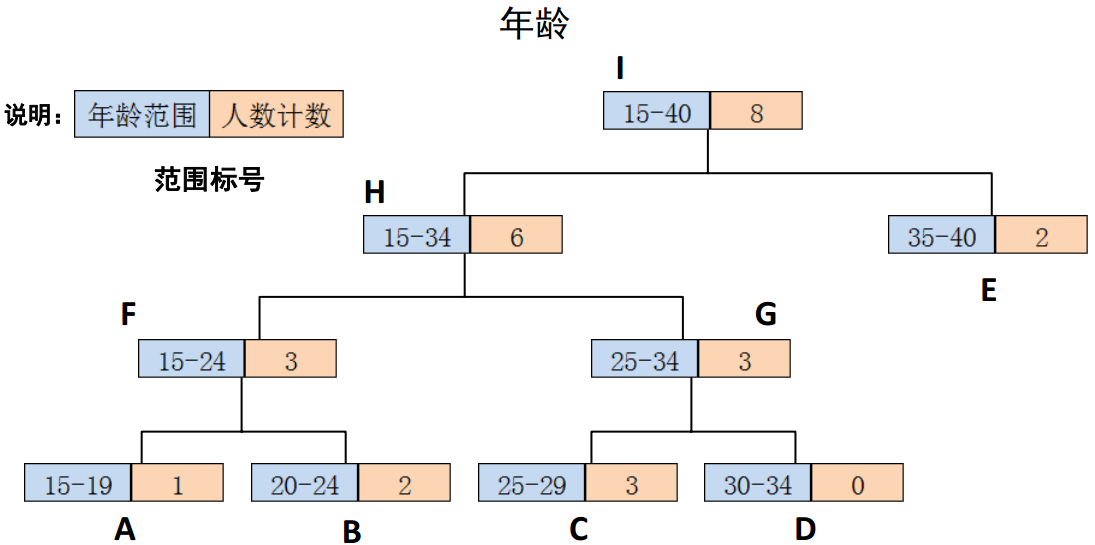
\includegraphics[width=5.5in]{chap4/examage}
	\bicaption[fig4:consistency]{图}{属性“年龄”的一致性树状结构}{Fig.}{The consistent tree structure for attribute 'Age'}
\end{figure}

\begin{exmp}
\label{chap4_exam}
数据集发布序列为叶节点数据项集合,即$\tilde{\mathcal{H}}$ = \{$\tilde{C}(x_{A})$,$\tilde{C}(x_{B})$,$\tilde{C}(x_{C})$,$\tilde{C}(x_{D})$,$\tilde{C}(x_{E})$\}。现有查询序列$\mathcal{Q}$=\{C([15-19]),C([20-29]),C([15-34]),C([15-40])\}。那么,对于单位长度查询C([15-19]),直接返回节点A的计数值$\tilde{C}(x_{A})$即可。对于范围查询C([20-29]),由于节点B,C的最小公共祖先节点集为{B,C},因此返回($\tilde{C}(x_{B})$+$\tilde{C}(x_{C})$);对于C([15-34]),其覆盖节点A,B,C,D的最小公共祖先节点集为{H},因此返回$\tilde{C}(x_{H})$;对于C([15-40],同理寻得A,B,C,D,E的最小公共祖先节点集为{I},返回$\tilde{C}(x_{I})$。
\end{exmp}

这是个树结构上的“最小集合覆盖”问题——寻找最小的能够完全覆盖给定的叶节点集合的父节点集。基于贪心思想,$DTree$树结构的最小集合覆盖算法TMSC描述如下:

\begin{algorithm}[H]
	\caption{基于$DTree$树结构的最小集合覆盖算法TMSC}
	\label{msc}
	\begin{algorithmic}[1]
		\REQUIRE $DTree$树结构, 待查询的属性范围$\mathbb{A}$
		\ENSURE 最小覆盖集合$\Upsilon$
		初始化 $\Upsilon$, $\Upsilon$ $\leftarrow$ $\varnothing$
		\FOR{后续遍历$DTree$中的每个叶节点$leaf$}
		\STATE $leaf$的覆盖范围表示为$cover(leaf)$
		\WHILE{$cover(leaf)$ $\subseteq$ $\mathbb{A}$}
		\STATE $leaf_{copy}$ $\leftarrow$ $leaf$
		\STATE $leaf$ $\leftarrow$ $leaf$的父节点
		\ENDWHILE 
		\STATE $\Upsilon$ $\leftarrow$ $\Upsilon$ $\bigcup$ $leaf_{copy}$
		\STATE $\mathbb{A}$ $\leftarrow$ $\mathbb{A}$ $-$ $cover(leaf_{copy})$
		\IF{$\mathbb{A}$ = $\varnothing$}
		\RETURN $\Upsilon$
		\ENDIF
		\ENDFOR
	\end{algorithmic}
\end{algorithm}

算法\ref{msc}中,属性范围$\mathbb{A}$为待覆盖集合,返回集合$\Upsilon$为最小的覆盖集合。算法第2行,后序遍历中仅对叶节点做处理。算法第3-6行,对于覆盖范围包含于集合$\mathbb{A}$的每个叶节点,贪心地向上取尽可能靠近根节点的父节点。第8,9行做更新处理。第10行,当$\mathbb{A}$为空,则表示$\Upsilon$中的节点集已经完全覆盖初始的$\mathbb{A}$,返回即可。

基于TMSC查询应答模式的数据发布格式初步方案,在\ref{LP_publish}节中已探讨过其利弊:(1)加噪后的$DTree$丧失一致性特性等式关系。(2)泄露了非叶结点的信息,隐私保障力度降低。
因此,后文介绍的DiffConOpt算法将对噪音分布进行调整,使得含噪的$DTree$重获一致性特性。因此,采用简单的直方图发布格式$\mathcal{H}$即可,通过单位长度数据项(叶节点)的叠加运算也能无差别地获取任意范围长度的数据项(非叶子节点),而不需暴露非叶结点信息。
%从而满足$TMSC$算法中返回父节点计数值的需求。

\subsubsection{重定义全局敏感性}

查询应答方式的改变引起了全局敏感性的改变,因此需要重新定义。

\begin{prop}
	\label{DTreeSensitivity}
	基于$DTree$的查询应答方式的全局敏感性为其树高$TH$。
\end{prop}
\begin{proof}
	见附录\ref{proof}。
\end{proof}

由于敏感性的改变,根据命题\ref{DTreeSensitivity}与全节点的发布格式,初步发布格式$\tilde{L}_{all}$基于拉普拉斯机制的差分隐私算法具体化为:
\begin{equation}
\label{chap4_dtree}
\tilde{L}_{all}(D) = L_{all}(D) + \textit{Laplace}(TH/\varepsilon)^{ntree}
%\widetilde{\mathcal{H}}(D) = \mathcal{H}(D) + \textit{Laplace}(TH/\varepsilon)^n
\end{equation}
其中,$ntree$为发布序列$\tilde{L}_{all}$的维度,即$DTree$的节点总数。

一般地有$TH$>1,可见此时由于全局敏感性的增加,在叶节点上添加了更大量级的拉普拉斯噪音。因此,TMSC应答查询模式在给非单位长度的范围查询带来效益的同时,可能会降低单位长度查询结果的准确性。下节介绍的算法DiffConOpt能够有效地解决这个问题,它高效地调整噪音分布,哪怕在单位长度查询准确度上的表现依旧优于直方图发布方式。

%从误差方差或者表达式方面与原来的式子进行比对 否则太粗糙了


%引出树的敏感性,小波和boost里边有,给出定义;研究下DiffGen的敏感性

%给图说明新的应答模式

%应说清 为了利用一致性进行应答,因此全局敏感要改,但是还是落在叶节点上。

\subsection{噪音分布调整算法DiffConOpt及最优化目标式}

$DTree$节点间的一致性特性是由匿名树泛化关系所决定的节点之间的固有属性,噪音的扰动仅仅是打破了数值等式关系,因此在确保总噪音量不缺失情况下,一致性特性是作为噪音数值调整的依据。
噪音调整算法DiffConOpt在DiffCon算法流程中具有三方面作用:(1)经过噪音分布调整后的$DTree$在节点计数值上重获一致性等式关系,这是采用直方图数据发布格式支持TMSC查询应答模式的前提。(2)能够使得整体的噪音分布更加“平滑”,每个节点的噪音量分布尽可能均匀。因此,无论对于单位长度的查询还是范围查询,均能提升查询结果的准确度。(3)不失隐私保障力度,保护了$DTree$内部节点的信息安全与联系。

假设$DTree$中的节点$x$的加噪计数表示为$\tilde{x}$,即"LapNoise"变量;调整后的优化结果为$\ddot{x}$,即"OptNoise"变量,中间变量记为$\acute{x}$。以节点$x$为根节点的子树中,其节点总数为$N_{total}(x)$,有$N_{leaf}(x)$个叶节点。$x$的父节点为$P_{x}$,$x$的下一层子节点集合为$ChildSet(x)$。
以下是DiffConOpt具体的实现算法\ref{adjustnoise}。

\begin{algorithm}[H]
	\caption{噪音调整算法DiffConOpt} 
	\label{adjustnoise}
	\begin{algorithmic}[1]
		\REQUIRE $DTree$树
		\ENSURE 重获一致性特性且优化噪音分布的$DTree$树
		\FOR{后续遍历$DTree$中的每个节点$x$}
		\IF{ $x$是叶节点}
		\STATE $\acute{x}$ $\leftarrow$ $\tilde{x}$ 
		\ELSE
		\STATE  $\acute{x}$ $\leftarrow$ $\frac{{N_{leaf}(x) * \tilde{x} + (N_{total}(x) - N_{leaf}(x)) * \sum\nolimits_{v \in ChildSet(x)} {\ddot{v}}}}{{N_{total}(x)}}$
		\ENDIF
		\ENDFOR
		\FOR{先序遍历$DTree$中的每个节点$x$}
		\IF{ $x$是根节点}
		\STATE  $\ddot{x}$ $\leftarrow$ $\acute{x}$
		\ELSE
	%	\STATE  $ChildNum$ = ${\sum\nolimits_{v \in Child(x)} {1}}$
		\STATE  $\ddot{x}$ $\leftarrow$ $\acute{x} + \frac{{\ddot{P_{x}} - \sum\nolimits_{v \in ChildSet(P_{x})} {\acute{v}}}}{|ChildSet(P_{x})|}$
		\ENDIF
		\ENDFOR
		\RETURN $DTree$
	\end{algorithmic}
\end{algorithm}

通过两次遍历完成算法DiffConOpt。第一次在算法第1行,自底向上的顺序遍历$DTree$的每个节点,求其优化结果。若非叶节点,则进行第5行的调整处理,否则直接以噪音值作为优化值。第二次采用自顶向下的顺序遍历节点,算法第8行开始,对于非根节点进行第12行的调整处理,否则原值返回;$|ChildSet(P_{x})|$表示集合$ChildSet(P_{x})$的大小,即$P_{x}$的下一层子节点总数。最后,发布重获一致性特性且具有更优噪音分布的$DTree$树。对于调整后的噪音分布,在算法\ref{diffcon1}的第5行,可具体化为$LapNoise$ $\leftarrow$ Laplace($TH$/$\varepsilon$)。

算法\ref{adjustnoise}对$BoostH$的完全$k$-叉树情况做了扩展,适用于任意树结构,其核心的噪音分布调整公式满足最小二乘法目标式,根据一致性约束条件,其最终形式为一线性规划式。DiffConOpt算法是优化途径,基于一致性约束的最小二乘法目标式是结论,命题\ref{chap4_consistent}在数学角度对二者的联系进行了描述。这也是DiffCon优化算法的理论核心,创新点和优化效果表述的体现,并在附录\ref{proof}中予以算法优化目标的正确性证明。

\begin{prop}
	\label{chap4_consistent}
	对于$DTree$上的每个节点$x$,经过式子
	\[
	\ddot{x} = \left\{ 
	{\begin{array}{*{20}l}
		\acute{x},  & {\begin{array}{*{20}l}
			x\text{为叶节点},   \\
			\end{array} }   \\ 
		
		\acute{x} + \frac{{\ddot{P_{x}} - \sum\nolimits_{j \in ChildSet(P_{x})} {\acute{j}}}}{|ChildSet(P_{x})|},  & {\begin{array}{*{20}l}
			x\text{非叶节点}  \\
			\end{array} }  \\  
		\end{array} } \right.
	\]
	后,得每个节点的优化值$\ddot{x}$满足基于一致性约束的最小二乘法目标式
	\begin{equation}
	\label{equa_l2}
	\begin{split}
	minimize \sum\limits_{x \in DTree} (\ddot{x} - \tilde{x})^2 \\
	subject\ \ to\ \ \forall x,\ \ \ddot{x} = \sum\limits_{c \in ChildSet(x)} \ddot{c} 
	\end{split}
	\end{equation}
\end{prop}
\begin{proof}
	见附录\ref{proof}。
\end{proof}

命题\ref{chap4_consistent}说明了DiffCon算法的理论基础,是一个从全节点分布角度出发的最优化问题。它从整体角度考虑每个节点上的噪音距离平方值,通过一致性约束条件追求最小化极值,从而达到优化噪音误差方差的目的。

\subsection{主要类图展示}
\label{chap4_class}
继上文对DiffCon算法每个部分设计与实现的介绍,本节通过主要的类图关系说明具体的实现细节,描述主要变量及函数的使用。虚线表示类之间的依赖关系,实线表示直接关联,如图\ref{fig4:class}所示。
\begin{figure}[!htp]
	\centering
	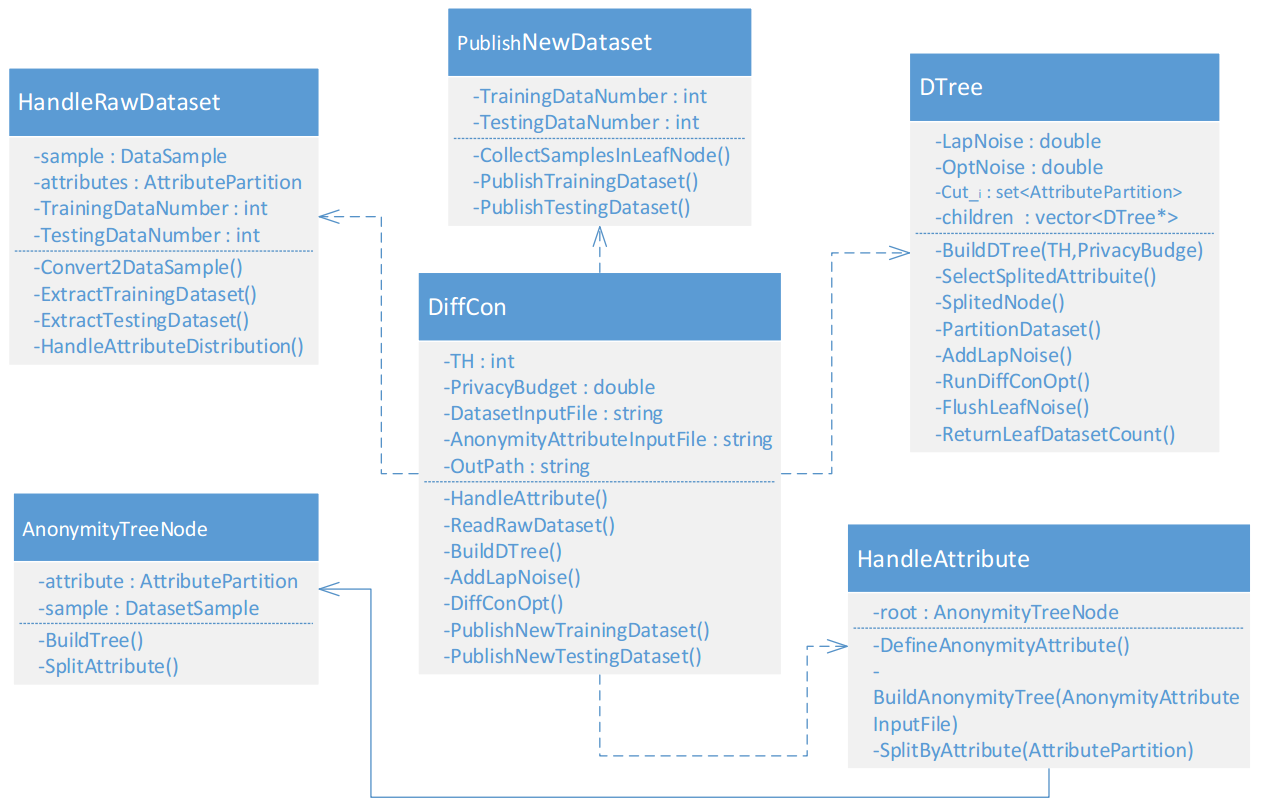
\includegraphics[width=6in]{chap4/class}
	\bicaption[fig4:class]{图}{DiffCon算法的主要类图展示}{Fig.}{The presentation of primary class diagram in DiffCon}
\end{figure}

以下对各类的功能和实现细节进行介绍:
\begin{enumerate}
	\item 算法主体为DiffCon类,变量DatasetInputFile记录原数据集位置,OutPath为输出的新数据集,AnonymityAttributeInputFile为自定义的匿名树语义文件,其中包括每种属性的匿名树定义。在函数部分,根据前文算法整体运行流程的介绍,展示了主要的函数,分别为原数据集属性处理函数(构建匿名树森林)、原数据集的数据项处理函数、构建$DTree$函数、加噪函数、优化算法DiffConOpt的实现函数、发布新数据集函数。
	\item HandleAttribute类对匿名树语义文件进行处理,建立属性的分裂规则。root变量为匿名树的根节点,因此我们为每个属性开辟独立的root空间,所有的匿名树构成root集合。SplitByAttribute函数根据参数按照划分规则对属性值进行切分操作。
	\item AnonymityTreeNode类为匿名树的节点定义。每个节点上有变量attribute和sample,它们维护了属性值节点与归属于此节点的数据集之间的对应关系,是操作$Cut_{i}$和指导$DTree$节点分裂的关键变量。
	\item HandleRawDataset类处理原数据集,根据比例划分为训练数据集与测试数据集,供后续的分类应用测试(实验章节)使用。Convert2DataSample函数读取并组织文件中的数据条目到内存,HandleAttributeDistribution函数数据集的属性分布。
	\item DTree类是$DTree$树结构的主要实现类,是伪代码\ref{diffcon2}的具体实现。参照伪代码,各函数的主要功能可通过函数名得知,此处不再重复介绍。
	\item PublishNewDataset类的主要作用是转换叶节点数据集为发布数据集。对应于HandleRawDataset类的处理,我们基于同一$DTree$结构,由划分的训练数据集和测试数据集最终得到相应的训练数据发布集与测试数据发布集,在实验章节通过真实的分类器测试算法性能。CollectSamplesInLeafNode函数负责统计叶节点数据分布情况,其余的两个函数实现训练/测试数据集的发布。
\end{enumerate}

\section{理论性能分析}
\label{theory analysis}

在DiffGen算法的噪音分布中,由于拉普拉斯加噪是个随机过程,导致噪音与真实值之间的“抖动性”——某些节点上的噪音与真实值相差巨大,某些却差距甚小。这种不均衡的噪音分布对噪音误差方差带来了巨大影响。经过算法DiffConOpt的调整,噪音分布不仅具有一致性关系,而且分布“平滑”。根据命题\ref{chap4_consistent}的最优化目标式,保证了噪音与真实值距离的总平方和最小,噪音的整体分布更加均匀。本节通过噪音误差方差对性能进行量化分析。

对于查询请求$\mathcal{Q}$中的第i个查询项,我们记\ref{linear_error}式的直方图发布方式的误差方差为$error_{Histog}^{\mathcal{Q}_{i}} = \frac{2|y_{i}-x_{i}|}{\varepsilon^2} = O(\frac{|y_{i}-x_{i}|}{\varepsilon^2})$。对于整个请求$\mathcal{Q}$,其误差方差为$error_{Histog}^{\mathcal{Q}}$
\begin{equation}
\label{linear_error2}
error_{Histog}^{\mathcal{Q}} = O(\frac{\sum\limits_i |y_{i}-x_{i}|}{\varepsilon^2})
\end{equation}

%在初步方案$\tilde{L}_{all}$中,
现在采用基于TMSC算法的应答查询模式,对于范围查询$\mathcal{Q}_{i}$,假设$TMSC$算法返回的集合$\Upsilon$=$\{a_{1},a_{2},...,a_{\Upsilon n}\}$。
在初步的数据发布方案$\tilde{L}_{all}$中,由误差方差定义有
\[
	error_{\tilde{L}_{all}}^{a_{j}} = \frac{2 \cdotp TH^2}{\varepsilon^2} = O(\frac{TH^2}{\varepsilon^2})
\]
其中 j = 1,2,..,$\Upsilon n$。

假设DTree中节点的最大分支数为$k$,那么$DTree$的节点总数$N_{total}$是与树高$TH$呈倍数关系,$N_{total}$ = $O(k \cdotp TH)$。例如完全三叉树时$N_{nodes}$ = $\Theta(3 \cdotp TH)$。因为经验公式及实际使用中,定义的匿名树的最大分支数通常都在个位数范围内,以防止通过决策树算法生成的分类树产生过度拟合(Overfitting)\supercite{overfitting}问题,而且基于决策树算法构建的$DTree$,分支数太多的属性值是很难被挑选到的。因此,在整个请求$\mathcal{Q}$中,集合$\Upsilon$在$\tilde{L}_{all}$上的误差方差$error_{\tilde{L}_{all}}^{\mathcal{Q}}$为

\[
\label{Lall_error}
error_{\tilde{L}_{all}}^{\mathcal{Q}} = \sum\limits_{j \in \Upsilon} error_{var}^{a_{j}}=O(\frac{TH^3}{\varepsilon^2})
\]

%1,说明单位长度也好。2,范围上的好处
现在讨论经过算法DiffConOpt优化后的应答查询模式,表示为$\tilde{\mathcal{H}}_{opt}$,其误差方差为$error_{\tilde{\mathcal{H}}_{opt}}^{\mathcal{Q}}$。

\begin{prop}
	\label{chap4_prop6}
	$error_{\tilde{\mathcal{H}}_{opt}}^{\mathcal{Q}} = O(\frac{TH^3}{\varepsilon^2})$
\end{prop}
\begin{proof}
	见附录\ref{proof}。
\end{proof}

进一步,比较$error_{\tilde{\mathcal{H}}_{opt}}^{\mathcal{Q}}$与$error_{\tilde{L}_{all}}^{\mathcal{Q}}$的大小关系。由于$k$仅仅表示最大分支数的取值,其他节点的分支数不确定,并且查询范围的细微区别也能使得应答集合$\Upsilon$大大不同,因此在大小比较与证明上通过$k$值和$TMSC$的最差应答策略取上届(Bound)关系式。

\begin{prop}
	\label{chap4_prop7}
	$error_{\tilde{\mathcal{H}}_{opt}}^{\mathcal{Q}} \leqslant \frac{3 \cdotp error_{\tilde{L}_{all}}^{\mathcal{Q}}}{2(k-1)(TH-2)+k}$
\end{prop}
\begin{proof}
	见附录\ref{proof}。
\end{proof}

由命题\ref{chap4_prop7}可以看到,经过噪音分布调整之后的$\tilde{\mathcal{H}}_{opt}$具有更好的误差方差,无论对于单位长度的查询还是范围查询而言,其查询结果均有更高的准确度,发布数据可用性更强。

\section{算法小结}

本章节对DiffCon算法的具体设计和实现进行了详细阐述,现在就算法运行流程和关键细节做分析总结。

首先,基于DiffGen分类树实现的$DTree$树是算法的结构基础,它呈现了各属性属性值间的匿名泛化关系及节点间的一致性联系,并且维护了“LapNoise”和“OptNoise”变量,为噪音优化算法DiffConOpt的运行做铺垫。

接下来,改变直方图发布方式的应答查询模式$LinearR$,通过基于树结构最小集合覆盖算法TMSC,设计新的查询应答模式,尽可能减少噪音叠加运算。之后重定义全局敏感性,并且在叶节点上添加拉普拉斯噪音以满足差分隐私。

DiffCon采用简单的一维直方图数据发布格式——基于单位长度数据项($DTree$的叶节点)。但由于加噪处理使得$DTree$节点间在数值上不再满足一致性等式,例如父节点的含噪计数值不等于其所有子节点的累加和。因此,需要对节点的噪音分布进行优化处理。基于核心调整公式,DiffConOpt算法对整体节点的噪音分布情况作一致性平衡调整。通过完整的基于一致性约束的最小二乘法目标式命题,给出算法优化目标及正确性的理论证明。

最后,采用DiffGen算法的发布方式——基于$DTree$的叶节点统计数据项,供范围计数查询类应用使用。

在性能探究方面,关注单位长度查询与范围查询两个角度。无乱是从本章节的理论角度还是下个章节的实验阶段,查询结果的准确度在DiffCon算法中均有所提升,并且在准确度扩展性、发布数据可用性上也有较大幅度的提高。


